\chapter{Corel Draw}

Beim Arbeiten mit Corel-Draw sind vor allem folgende Dinge zu beachten:

\begin{itemize}
  \item Noch viel mehr als bei den \LaTeX-Dokumenten sollte man hier auf
    {\bf copy-and-paste} bauen. Praktisch alle Symbole (Blöcke, Pfeile,
    Auflager, Federn, Dämpfer, etc.) können in bestehenden {\tt .cdr}-files
    gefunden werden. Würden eigene Symbole hierfür gezeichnet werde, so wäre das
    neue Bild nicht mehr konsistent mit den restlichen.
  \item Beim Abspeichern der {\tt .cdr}-files sollte man darauf achten, diese
    im {\bf Version 14} abzuspeichern. Dies rührt daher, dass die 
    Corel-Draw-Installation eines Rechners in der Institutsbibliothek maximal
    Version 14 öffnen. Arbeitet man auf dem anderen Rechner hat man darauf
    achten, dass dieser standardmäßig in höheren Versionen speichert!
  \item Die Nummerierung der Beispiele in der Formelsammlung (z.B.
    \twrite{C01.cdr}, etc.) geschieht zwar ohne wirkliches Muster, ist aber 
    keinesfalls beliebig! Dies soll an folgendem Beispiel erklärt werden: 
    Angenommen im Ordner des dritten Kapitels
    (\twrite{3\_kinetik eines Systems von MP}) befinden sich die Dateien 
    \twrite{C16.cdr}, \twrite{C17.cdr} und \twrite{C18.cdr}. Muss man nun in 
    diesem Kapitel ein neues Bild einfügen, so läge es nahe dies mit der Nummer
    19 (\twrite{C19.cdr}) auszustatten. Nun kann es aber durchaus sein, dass in 
    Kapitel 6 (\twrite{6\_schwingungen}) bereits ein Bild mit dem Namen
    \twrite{C19.cdr} existiert. Problematisch wird das Ganze, wenn
    man nun das Bild als {\tt .eps} exportiert: Zumal die {\tt .eps}-files
    aller Kapitel in dem selben Ordner sind, würde man das alte überschreiben.
    Um festzustellen ob ein Name in Verwendung ist oder nicht, kann man 
    Folgendes machen: Man erstellt das {\tt .cdr} mit dem gewünschten Namen
    und versucht es gleich als {\tt .eps} zu exportieren. Wenn man jetzt die 
    Warnung bekommt, dass ein {\tt .eps} mit dem Namen schon existiert, weiß 
    man, dass der Name schon vergeben ist, bricht die Exportierung ab und sucht
    einen neuen Namen. Dies ist der Grund wieso die Bezeichnung der Bilder in
    der Formelsammlung eher undurchsichtig ist: Teilweise werden Indizes 
    verwendet (z.B. \twrite{C19\_a.cdr}) oder auch der erste Buchstabe geändert
    (z.B. \twrite{D19.cdr}).
\end{itemize}

Im Folgenden wird noch auf ein paar Funktionen von Corel Draw eingegangen, die
sich vielleicht nicht sofort erschließen, aber sehr hilfreich sind.

\section{Objekteigenschaften}

Eine der wichtigsten Funktionen sind die Objekteigenschaften. Sie können durch
einen Rechtsklick, gefolgt durch anwählen des Buttons \twrite{Eigenschaften}
angezeigt werden. Alternativ kann man sie auch mit der Tastenkombination
\twrite{Alt + Enter} einblenden. Es gibt hier zwei wichtige Reiter, die im
Folgenden beschrieben werden:

\begin{itemize}
  \item {\bf Füllung} (Farbtopf-Symbol):\\
    Wie der Name schon sagt, kann hier die Farbe und der Verlauf der Füllung
    eingestellt werden (es gibt auch die Option {\tt keine Füllung}). Unter
    \twrite{Erweitert} findet man spezielle Muster, die aber eigentlich nicht
    gebraucht werden.
  \item {\bf Umriss} (Füllfeder-Symbol):\\
    Hier kann man einerseits die Stärke und Farbe der Linien festlegen,
    andererseits können aber auch die Pfeilspitzen editiert werden. Unter
    \twrite{Erweitert} findet man diese Optionen: Rechts oben können die
    Pfeile an beiden Enden mit \twrite{Optionen} verändert werden. Neben
    Befehlen wie {\tt Bearbeiten} oder {\tt Löschen}, gibt es das nützliche
    Kommando {\tt Tauschen}, welches die Pfeilspitzen der beiden Enden
    vertauscht. Dies ist nützlich, wenn man bei einen gekrümmten Pfeil (der z.B.
    ein Moment oder eine Winkelgeschwindigkeit repräsentiert) den Drehsinn
    ändern möchte.
\end{itemize}

In \figref{fig:objarrow} werden beide Reiter in einer Grafik dargestellt.

\begin{figure}[htbp]
  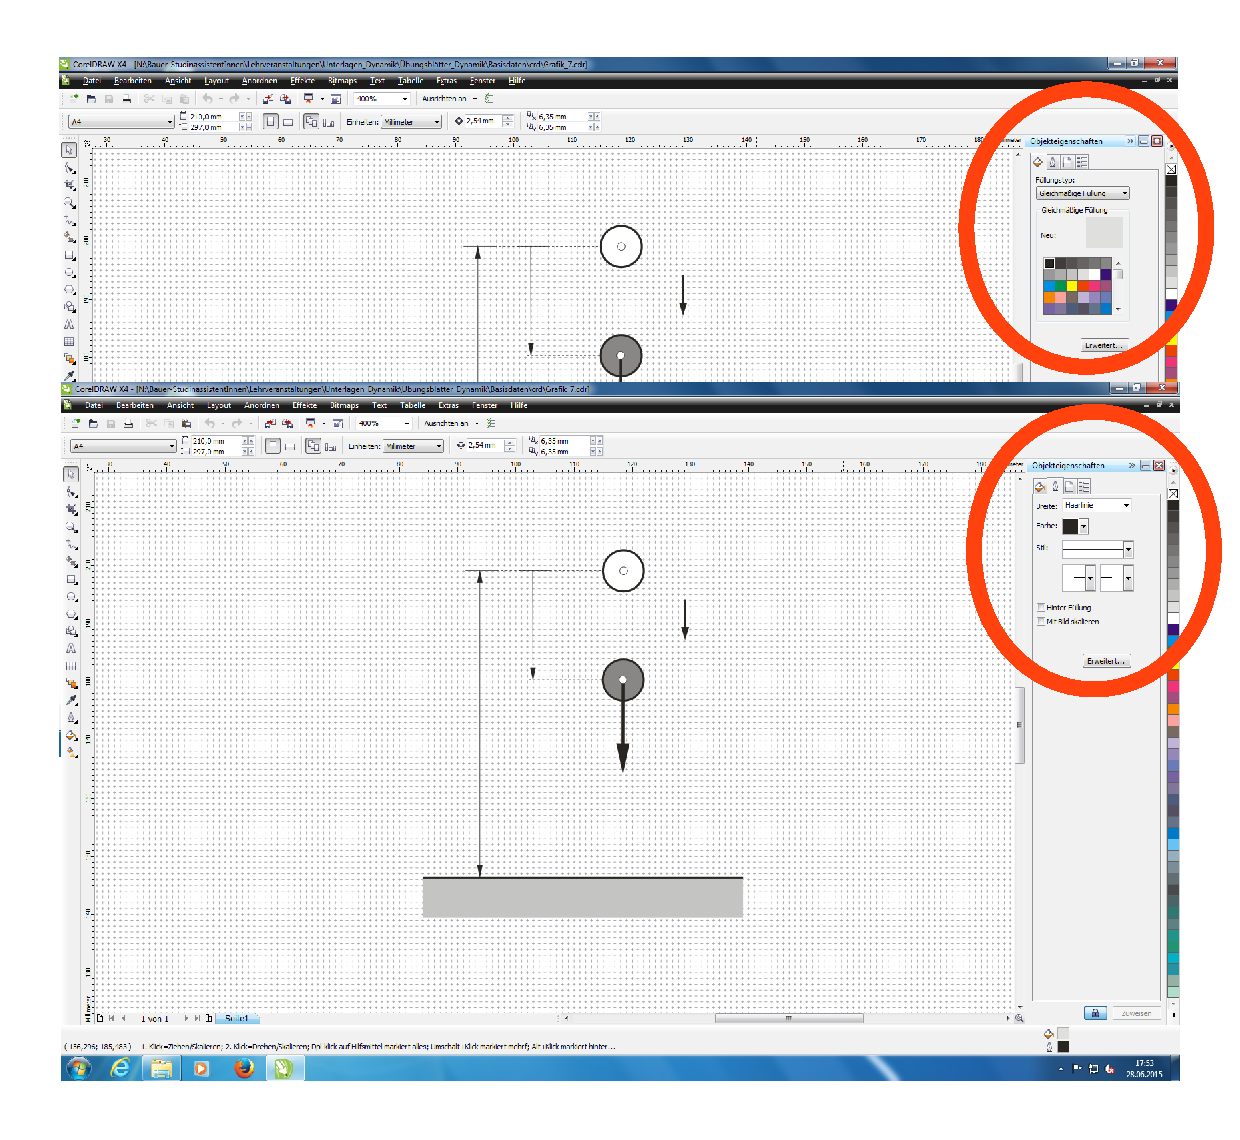
\includegraphics[width=\textwidth]{2_objeigen.pdf}
  \caption{Objekteigenschaften: {\bf Füllung} (oben) und {\bf Umriss} (unten).}
  \label{fig:objarrow}
\end{figure}

\clearpage
\section{Rotation}

Um ein Objekt zu drehen muss man es auswählen und dann noch einmal auf das
Objekt klicken. Es werden gekrümmte Pfeilchen an den Ecken eingeblendet und
der {\bf Rotationspunkt} (dieser ist äquivalent zum mechanischen Momentanpol
einer Bewegung) wird angezeigt. Dieser ist durch einen Kreis mit einem Punkt
darin gekennzeichnet und kann in Abbildung \figref{fig:rot} beobachtet werden.
Der Rotationspunkt lässt sich beliebig verschieben, was bei sehr vielen
Drehungen sehr nützlich ist. Das Objekt wird gedreht indem man einen der
gekrümmten Pfeilchen anwählt und das Objekt herumzieht. Alternativ kann in
der oben Aktionsleiste auch der Drehwinkel eingestellt werden.

\begin{figure}[htbp]
  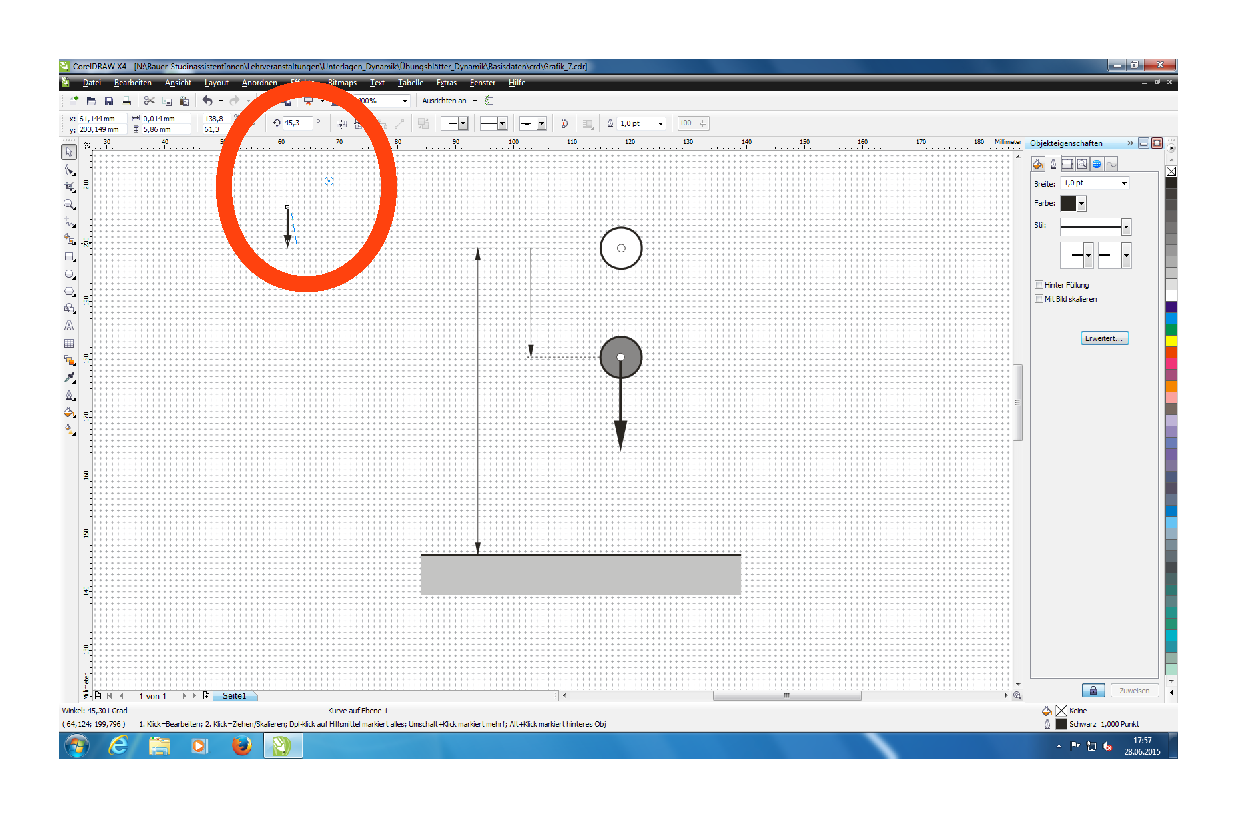
\includegraphics[width=\textwidth]{2_rot.pdf}
  \caption{Rotieren eines Objekts. Man beachte den Rotationspunkt (entspricht
   sozusagen dem Momentanpol der Bewegung). In dem durch die Ellipse markierten
   Bereich befindet sich auch die manuelle Einstellung des Drehwinkels in
   der Aktionsleiste (ganz oben in der Ellipse).}
  \label{fig:rot}
\end{figure}

\newpage
\section{Hilfsmittel \twrite{Form}}

Das Hilfsmittel \twrite{Form} dient, wie der Name schon suggeriert, zum Ändern
der Form eines Objekts. Es befindet in der linken Aktionsleiste, relativ weit
oben (siehe \figref{fig:form}). Das Tool wird vor allem dazu gebraucht, bei
Freiformen die Kontrollpunkte der Bezierkurven zu verschieben.

\begin{figure}[htbp]
  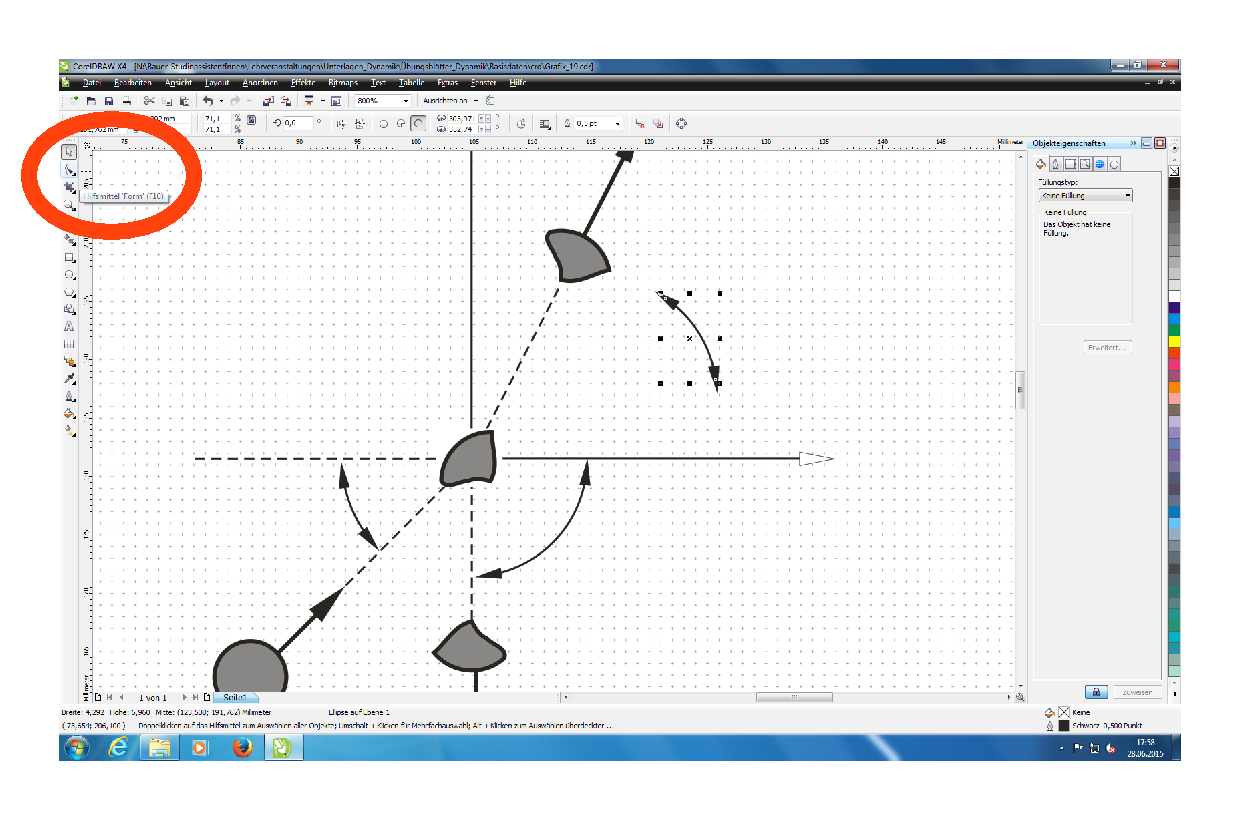
\includegraphics[width=\textwidth]{2_form.pdf}
  \caption{Tool Form.}
  \label{fig:form}
\end{figure}

Ein weiterer wichtiger Anwendungsfall von \twrite{Form} tritt im Zusammenhang
mit Kreissektoren auf. Grundsätzlich wird es dazu verwendet, um den 
Öffnungswinkel zu verändern. Es ist jedoch wichtig wo der Mauscursor
positioniert ist, wenn die Maustaste losgelassen wird. Befindet sich der Cursor
im Kreissegment, so wird das eigentliche Segment gezeichnet (berandet durch
einen Kreisbogen und zwei Geraden). Dieser Sachverhalt wird in 
\figref{fig:circlein} dargestellt. Ist aber der Cursor außerhalb des Segments,
wenn die Maustaste losgelassen wird, so wird nur der Kreisbogen gezeichnet,
inklusive Pfeile (sofern vorhanden), siehe \figref{fig:circleout}. 
Erstere Option eignet sich also, um wirkliche Kreissegmente 
(\glqq{}Tortenstücke\grqq{}) zu zeichnen, während letztere gebraucht wird, um 
Winkel einzuzeichnen.

\begin{figure}[htbp]
  \begin{center}
  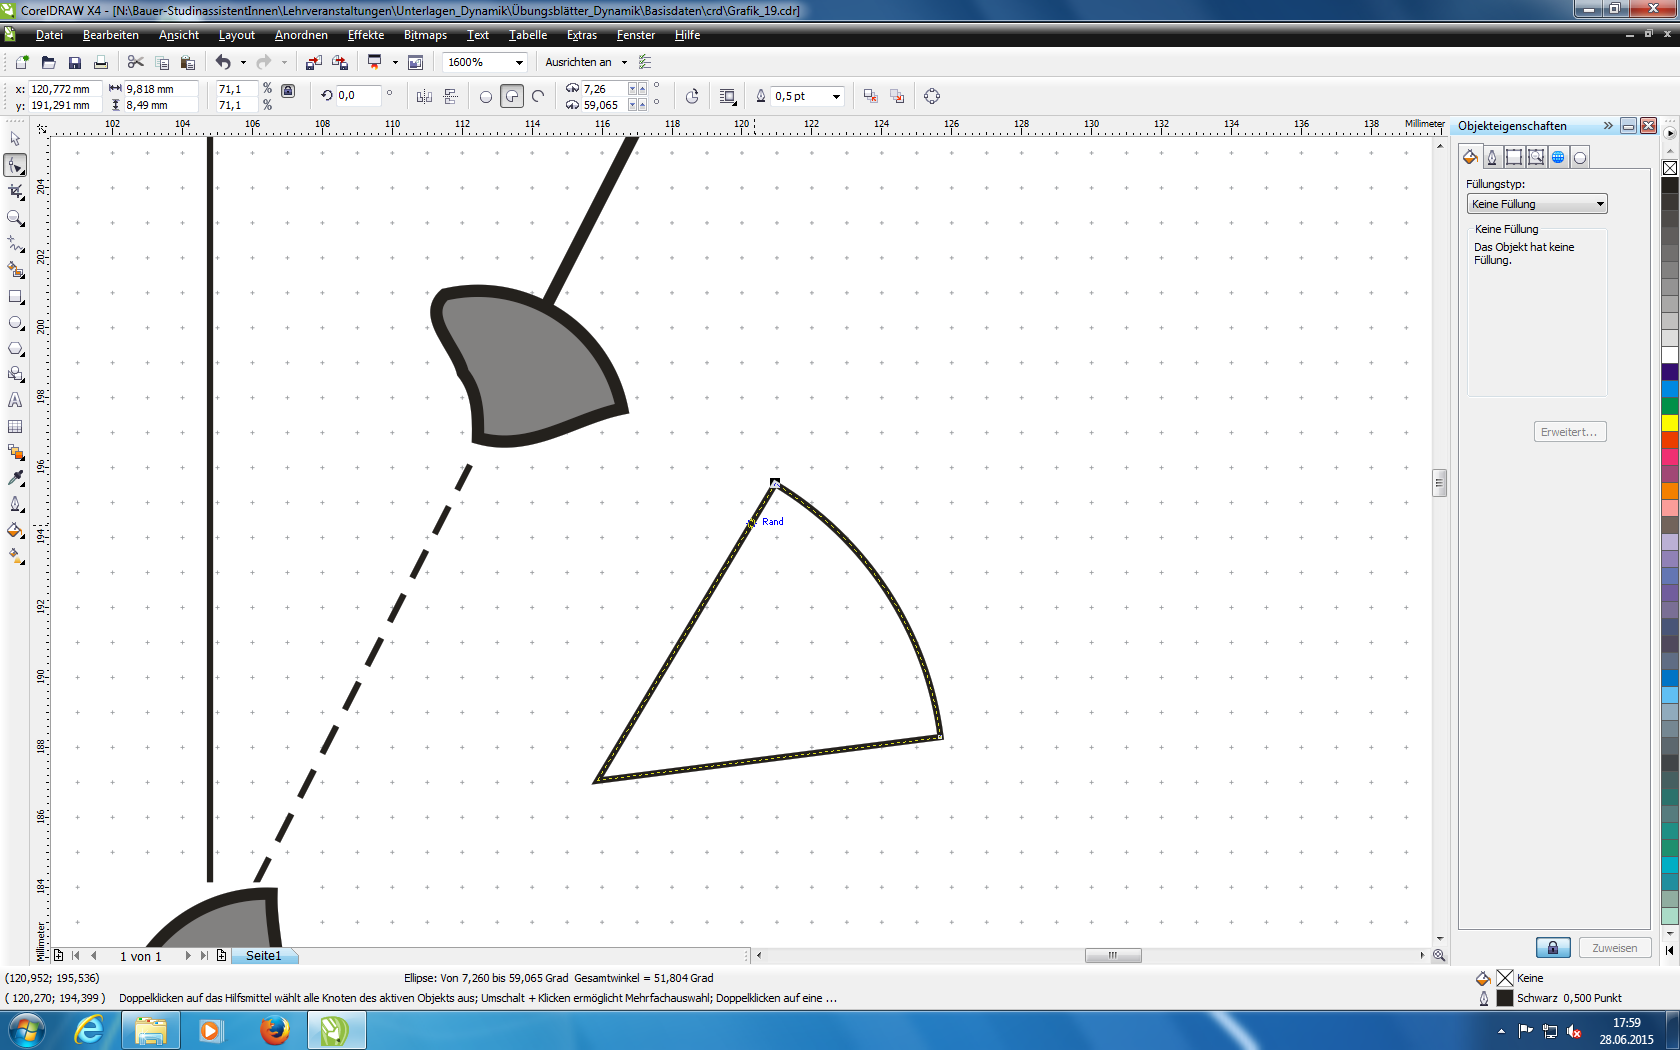
\includegraphics[width=.9\textwidth]{2_circle_in.png}
  \end{center}
  \caption{Tool \twrite{Form} angewendet auf einen Kreissektor. Der Cursor wird
   innerhalb des Segments losgelassen, wodurch das volle Segment (ohne
   Pfeilspitzen) gezeichnet wird.}
  \label{fig:circlein}
\end{figure}


\begin{figure}[htbp]
  \begin{center}
  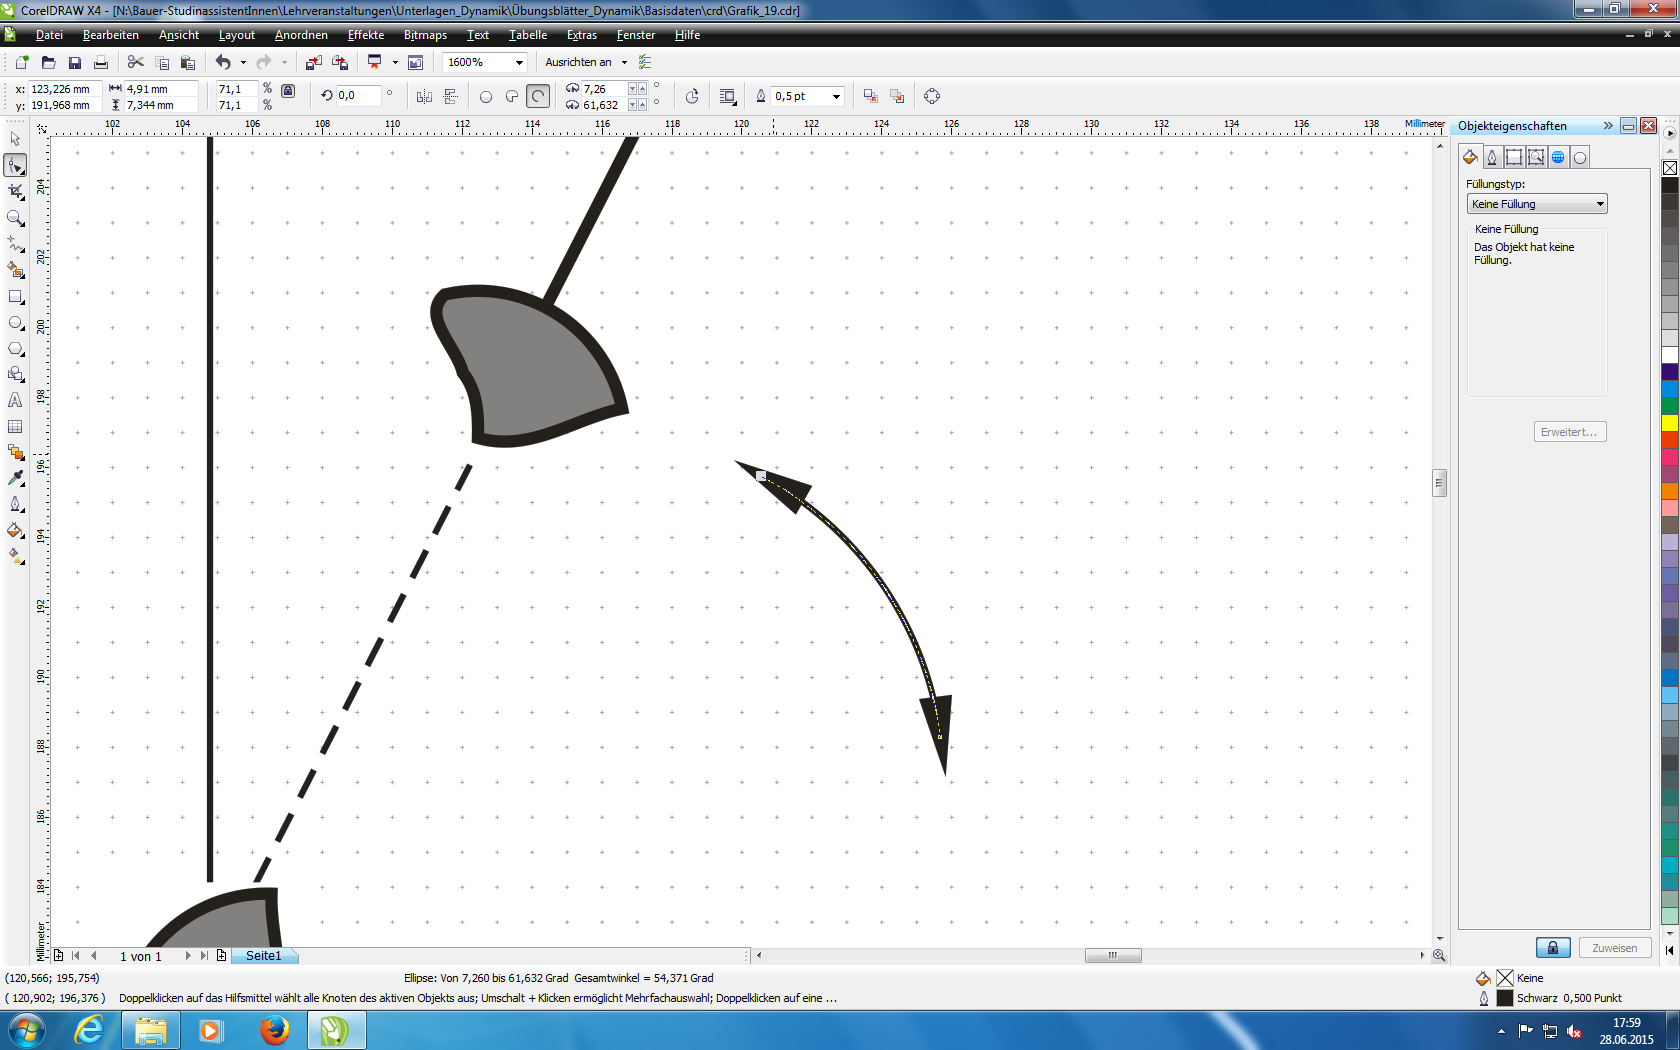
\includegraphics[width=.9\textwidth]{2_circle_out.png}
  \end{center}
  \caption{Tool \twrite{Form} angewendet auf einen Kreissektor. Der Cursor wird
   außerhalb des Segments losgelassen, wodurch nur der Kreisbogen (mit
   eventuell vorhandenen Pfeilspitzen) gezeichnet wird.}
  \label{fig:circleout}
\end{figure}

%EOF